\chapter{Retrieval and Optimization Methods}
\label{chap:retrieval_optimization}

The retrieval component constitutes the core of a RAG system. Its capacity to extract high-quality, pertinent information from an extensive corpus is the primary determinant of the system's overall performance. This chapter offers a comprehensive examination of the critical techniques employed to construct and optimize the retrieval pipeline, encompassing the initial processing of documents through to the final reranking of retrieved candidates. We will follow the structure proposed by Gao et al. (2024) \autocite{gao2024retrievalaugmentedgenerationlargelanguage}, which categorizes RAG optimization into pre-retrieval, retrieval, and post-retrieval stages.

\section{Chunking Techniques}
Chunking constitutes a crucial pre-retrieval processing step that entails segmenting large documents into smaller, more manageable units. The objective is to generate chunks that are semantically coherent and sufficiently compact to be efficiently processed by embedding models and accommodated within the context window of an LLM, as LLMs performance reduce drastically when irrelevant information is included \autocite{shi2023largelanguagemodelseasily}. The selection of a chunking strategy exerts a substantial influence on retrieval quality.

\subsection{Naive vs. Semantic Chunking}
\textbf{Naive Chunking}, also referred to as fixed-size chunking, represents the most straightforward approach. It entails segmenting documents into portions of a predetermined length (e.g., 200 words) with an optional overlap between contiguous chunks. While straightforward to implement, this method can prove suboptimal as it frequently bisects sentences or paragraphs, thereby disrupting the semantic continuity of the text. This can lead to a loss of crucial context, as a single concept might be split across multiple chunks, making it harder for the embedding model to capture its full meaning and for the LLM to synthesize a coherent answer.

\textbf{Semantic Chunking} constitutes a more sophisticated approach. Rather than depending on arbitrary lengths, it endeavors to delineate the text at logical boundaries. This can be accomplished through several methodologies:

\subsubsection{Sentence-Level Chunking}
Employing natural language processing libraries to segment the text into discrete sentences. This approach offers high granularity, making it easier to pinpoint exact sources for generated responses. However, it can result in a large number of very small chunks, which might lack sufficient context on their own, potentially leading to less informative embeddings if a concept spans multiple sentences.

\subsubsection{Recursive Chunking}
A hierarchical method that initially attempts to segment by larger logical units (e.g., paragraphs, sections), subsequently by smaller units (e.g., sentences), and ultimately by words, with the aim of preserving semantic coherence to the greatest extent feasible. This method is particularly effective for documents with clear structural hierarchies, as it prioritizes maintaining the integrity of semantic units. For instance, a document might first be split by double newlines (paragraphs), then by single newlines, then by sentences, and finally by characters if necessary, ensuring that chunks are as semantically complete as possible.

The choice of chunking strategy directly impacts the quality of the generated embeddings and, consequently, the retrieval performance. Chunks that are too small may lack sufficient context for the embedding model to accurately capture their meaning, leading to poor retrieval. Conversely, chunks that are too large might dilute the relevance of specific information, making it harder for the retriever to identify the most pertinent segments and increasing the risk of the "lost in the middle" problem for the LLM. An optimal chunk size balances contextual completeness with conciseness.

From a practical standpoint, various libraries and tools offer functionalities for implementing these chunking strategies. For instance, frameworks like LangChain \autocite{langchain} provide robust text splitters that support fixed-size, recursive, and other semantic-aware chunking methods. Natural Language Toolkit (NLTK) \autocite{loper2002nltknaturallanguagetoolkit} and SpaCy \autocite{honnibal2020spacy} are commonly used for sentence tokenization, which forms the basis for sentence-level chunking.

\section{Embedding Models}
The selection of an embedding model is paramount for accurately capturing the semantic meaning of the text. These models convert text into high-dimensional vectors, such that semantically similar texts are positioned in closer proximity within the vector space.

\subsection{Contextual Embeddings}
Contemporary RAG systems leverage \textbf{contextual embeddings}, exemplified by those generated by transformer-based models including BERT \autocite{devlin2019bertpretrainingdeepbidirectional}, RoBERTa \autocite{liu2019robertarobustlyoptimizedbert}, and the OpenAI Ada series. In contrast to earlier static word embeddings (e.g., Word2Vec, GloVe), which attribute a singular vector to each word, contextual embeddings produce a distinct vector for a word contingent upon the sentence in which it is situated. This enables them to capture linguistic nuances, ambiguity, and the richness of language, thereby facilitating more accurate semantic search. The underlying transformer architecture, with its self-attention mechanisms, allows these models to weigh the importance of different words in a sentence when generating an embedding for a specific word, thus capturing its meaning in context. This capability is crucial for tasks requiring a deep understanding of semantic relationships, such as information retrieval.

\subsection{Fine-tuning Embedding Models}
For domain-specific applications, pre-trained embedding models may not exhibit optimal performance. Fine-tuning the embedding model on a dataset representative of the target domain—augmented with synthetic examples—can substantially enhance retrieval relevance \autocite{gill2025advancingsemanticcachingllms}. As shown by Gill et al. (2025) \autocite{gill2025advancingsemanticcachingllms}, even compact embedding models fine-tuned for a single epoch on specialized and synthetically augmented datasets significantly outperform state-of-the-art alternatives in precision and recall.

\subsection{The MTEB Leaderboard}
The quality of embedding models is often evaluated using benchmarks that assess their ability to capture semantic similarity and perform retrieval tasks. Metrics such as Mean Average Precision (MAP), Recall@k, and Normalized Discounted Cumulative Gain (nDCG) are commonly used to quantify their performance on various datasets. A prominent resource for this evaluation is the Massive Text Embedding Benchmark (MTEB) leaderboard \autocite{mteb_leaderboard_2025}. MTEB comprehensively ranks over 100 text and image embedding models across more than 1000 languages, encompassing 131 tasks categorized into 9 task types (including BitextMining, Classification, Clustering, InstructionRetrieval, MultilabelClassification, PairClassification, Reranking, Retrieval, and STS). It also covers 20 diverse domains such as Academic, Financial, Legal, Medical, and News, providing a broad and highly-curated comparison of embedding model performance in various real-world scenarios.
\subsection{Evaluated Embedding Models}
In this thesis, we evaluate the performance of several prominent embedding models.
A detailed experimental comparison and analysis of these models are presented in Chapter \ref{chap:experiments_results}, Section \ref{sec:exp_embedding_models}.

\subsubsection{OpenAI \texttt{text-embedding-ada-002}:} A widely adopted, high-performance proprietary model with a vector size of 1536. This model unifies five separate models (for text search, text similarity, and code search) into a single model, outperforming its predecessors at most tasks. It features an increased context length from 2048 to 8192 tokens and a smaller embedding size of 1536 dimensions, making it more cost-effective \autocite{openai2022ada002}.

\subsubsection{Nomic AI \texttt{nomic-embed-text}:} An open-source model possessing a vector size of 768. This model is notable as the first fully reproducible, open-source, open-weights, and open-data English text embedder with an 8192 context length. It outperforms OpenAI Ada-002 and text-embedding-3-small on both short and long-context benchmarks. It employs a prefix for distinct tasks: \texttt{search\_query} for queries and \texttt{search\_document} for documents in retrieval tasks \autocite{nussbaum2025nomicembedtrainingreproducible}.

\subsubsection{Jina AI \texttt{jina-embeddings-v2-base-en}:} An open-source model with a vector size of 768. This model, like Ada-002, does not require a task instruction. This model is notable for its ability to accommodate up to 8192 tokens, transcending the conventional 512-token limit by employing a modified BERT architecture with bi-directional ALiBi slopes for positional information. Its training involves three stages: pre-training a modified BERT, fine-tuning with text pairs, and fine-tuning with hard negatives. It matches the performance of OpenAI's \texttt{text-embedding-ada-002}, making it suitable for efficiently processing long documents and addressing fragmented semantic meanings caused by traditional chunking \autocite{günther2024jinaembeddings28192token}.

\subsubsection{Jina AI \texttt{jina-embeddings-v3}:} The successor of jina-embeddings-v2 embedding model with 570 million parameters, optimized for multilingual data, long-context retrieval, and high performance across multiple tasks. It introduces task-specific Low-Rank Adaptation (LoRA) adapters to generate high-quality embeddings for various tasks. This model implements \textit{late chunking}, where chunks from the same document are tokenized together up to the model's context window of 8192 tokens, with a vector size of 1024. It requires a \texttt{task} argument: \texttt{retrieval.query} and \texttt{retrieval.passage} for queries and documents respectively. It outperforms recent proprietary embeddings from OpenAI and Cohere on English tasks, and multilingual-e5-large-instruct across all multilingual tasks, offering a more cost-efficient solution \autocite{sturua2024jinaembeddingsv3multilingualembeddingstask}.

\subsubsection{Qwen \texttt{Qwen3-Embedding-0.6B}:} An open-source model with a vector size of 1024. This model is part of the Qwen3 Embedding series, built upon the Qwen3 foundation models. It leverages the robust multilingual text understanding and generation capabilities of Qwen3 LLMs through an innovative multi-stage training pipeline that includes large-scale unsupervised pre-training and supervised fine-tuning. It achieves state-of-the-art results across diverse benchmarks, particularly excelling on the MTEB Multilingual benchmark. This model benefits from a prompt for queries, for which we used the recommended \texttt{query} prompt name \autocite{zhang2025qwen3embeddingadvancingtext}.

\section{Post-Retrieval Reranking and Filtering}
Subsequent to the initial retrieval of documents based on semantic similarity, their relevance and ordering can be further refined through post-retrieval processing. This constitutes a pivotal component of the \textbf{Advanced RAG} paradigm \autocite{gao2024retrievalaugmentedgenerationlargelanguage}.

\subsection{BM25 and TF-IDF for Reranking}
Traditional information retrieval algorithms, such as Best Match 25 (BM25) \autocite{robertson1995okapi} and Term Frequency - Inverse Document Frequency (TF-IDF) \autocite{td-idf_sparck, salton1975vector}, are predicated on keyword matching. They demonstrate high efficacy in identifying documents that contain the precise keywords from the query. While dense retrievers (vector search) ascertain the user's semantic intent, these sparse retrievers identify the user's explicit lexical terms. BM25, specifically, is a ranking function that estimates the relevance of documents to a given search query. It improves upon TF-IDF by incorporating document length normalization and term frequency saturation, which prevents very long documents or documents with very high term frequencies from being disproportionately ranked.

\begin{equation}
\text{BM25}(q,d) \;=\; \sum_{i=1}^{|q|} \! \mathrm{IDF}(q_i)\; 
  \frac{f(q_i,d)\,(k_1+1)}{f(q_i,d) + k_1\bigl(1 - b + b\,\frac{|d|}{\mathrm{avgdl}}\bigr)}
\label{eq:bm25}
\end{equation}

where $f(q_i,d)$ is the term frequency of query term $q_i$ in document $d$, $|d|$ is the length of $d$, $\mathrm{avgdl}$ is the average document length in the collection, and $k_1,b$ are tuning parameters \autocite{robertson1995okapi}. IDF is typically defined as

\[
  \mathrm{IDF}(t) = \ln\!\biggl(\frac{N - n_t + 0.5}{n_t + 0.5} + 1\biggr),
\]
with $N$ the total number of documents and $n_t$ the number of documents containing term $t$.

By contrast, TF–IDF scores a term $t$ in document $d$ as the product of its normalized frequency and its inverse document frequency:
\begin{equation}
\text{TF–IDF}(t,d,D) \;=\;
  \underbrace{\frac{f(t,d)}{\sum_{t'} f(t',d)}}_{\displaystyle\mathrm{TF}(t,d)}
  \;\times\;
  \underbrace{\log\!\Bigl(\frac{|D|}{|\{d'\in D: t\in d'\}|}\Bigr)}_{\displaystyle\mathrm{IDF}(t,D)}
\label{eq:tfidf}
\end{equation}
where $f(t,d)$ is the raw count of term $t$ in $d$, $|D|$ the total number of documents, and the denominator counts those documents in which $t$ appears \autocite{salton1975vector,td-idf_sparck}.

By employing BM25 or TF–IDF to rerank the candidates retrieved via vector search, performance can be enhanced through the elevation of documents exhibiting substantial lexical overlap with the query \autocite{gao2024retrievalaugmentedgenerationlargelanguage}. This hybrid approach leverages the strengths of both semantic (dense) and keyword (sparse) matching.

\subsection{Hybrid Systems: Combining Similarity with BM25/TF-IDF}
A \textbf{hybrid system} integrates the scores derived from both dense (embeddings-based methods) and sparse (BM25 or TF-IDF) retrieval methods. A prevalent approach involves utilizing a weighted combination of scores from a vector search and a BM25 search to yield a final relevance score. This enables the system to capitalize on the strengths of both approaches, thereby encompassing both semantic relevance and keyword importance for a more robust retrieval process \autocite{gao2024retrievalaugmentedgenerationlargelanguage}.

\subsection{Cross-Encoder Rerankers}
For maximal accuracy, a \textbf{cross-encoder} model can be employed as a final reranking step \autocite{nogueira2019passage}. In contrast to bi-encoders (standard embedding models) that generate distinct embeddings for the query and documents independently, a cross-encoder processes the query and a candidate document as a unified input. This allows the model to perform a deep, token-by-token comparison between the query and the document, yielding a highly precise relevance score \autocite{khattab2020colbertefficienteffectivepassage}. This "cross-attention" mechanism enables the model to capture intricate relationships and subtle nuances that might be missed by bi-encoders. However, cross-encoders incur significant computational expense due to the need to process each query-document pair, making them generally reserved for reranking a limited number of top candidates (typically 50-200) from a more rapid, initial retrieval stage. Their use may be justified in applications where high precision and relevance are paramount, even at the cost of increased latency.

\section{Dynamic Similarity Thresholding}
Rather than retrieving a predetermined number of chunks (top-N), \textbf{dynamic similarity thresholding} adjusts the retrieval process based on the query itself. For certain queries, only a limited number of highly relevant chunks may be requisite, whereas for others, a more expansive context proves advantageous. Dynamic thresholding methods analyze the distribution of similarity scores for a given query and endeavor to identify a natural cutoff point, thereby facilitating the retrieval of a more contextually appropriate number of chunks. This precludes the inclusion of irrelevant documents when similarity scores exhibit a sharp decline and permits more comprehensive retrieval when numerous documents demonstrate comparable relevance. The traditional approach of retrieving a fixed number of top-N documents (e.g., the top 5 most similar chunks) may prove suboptimal. A fixed N fails to account for the varying relevance distribution across different queries. For a highly specific query, only one or two documents might be truly relevant, and retrieving more would introduce noise. Conversely, for a broad query, a larger set of documents might be necessary to provide a comprehensive answer. Furthermore, a fixed N can exacerbate the "lost in the middle" problem, where relevant information might be overlooked by the LLM if it's buried within a large context window filled with less relevant chunks. Dynamic thresholding aims to retrieve precisely the right amount of information, optimizing for both precision and recall.

\subsection{Methods for Dynamic Thresholding}
Several approaches can be employed to implement dynamic similarity thresholding. In our experiments, we specifically evaluated the following methods:

\subsubsection{Statistical Methods}
These methods analyze the statistical properties of the similarity scores for a given query. For instance, one could set a threshold based on a certain number of standard deviations from the mean similarity score, or by identifying a significant drop-off in scores. A common example is \textbf{Percentile} thresholding, where a fixed percentile of the ranked scores is chosen as the cutoff. While straightforward, this method often included an excessive number of documents, as observed in our experiments (Table \ref{tab:merged_retrieval_stats}), leading to diluted context.

\subsubsection{Distribution-based Methods}
These approaches examine the distribution of similarity scores to find natural cut-off points. Techniques evaluated include:
\begin{itemize}
    \item \textbf{Gaussian Mixture Models (GMM):} This method attempts to model the distribution of similarity scores as a mixture of Gaussian distributions, typically two (one for relevant, one for irrelevant), and sets the threshold at the point where the probability of belonging to the "relevant" distribution drops significantly. Our experiments showed GMM often included a very high number of items, similar to Baseline, resulting in low F1 scores (Table \ref{tab:reranker_performance}).
    \item \textbf{Knee:} This method identifies the "knee" or "elbow" point in the sorted similarity scores, where the rate of change in scores significantly decreases. This point is often considered an optimal balance between including enough relevant items and avoiding diminishing returns. Knee thresholding showed improved F1 scores over GMM and Otsu in our experiments, indicating a better balance.
    \item \textbf{Max Gap:} This method identifies the largest difference between consecutive similarity scores when sorted in descending order. The threshold is set at the score immediately preceding this largest gap, assuming it represents a clear separation between relevant and less relevant documents. In our experiments, Max Gap consistently yielded the highest F1 scores, particularly when combined with effective rerankers, by selecting a compact and highly relevant set of documents (Table \ref{tab:reranker_performance}).
    \item \textbf{Otsu:} Originally developed for image thresholding, Otsu's method can be applied to similarity scores to find a threshold that minimizes the intra-class variance of the two groups (below and above the threshold) or, equivalently, maximizes the inter-class variance. Similar to GMM, Otsu often resulted in including a large number of documents in our experiments, leading to low F1 scores.
    \item \textbf{2nd Derivative:} This method identifies inflection points in the sorted similarity score curve by analyzing its second derivative. A significant change in the curvature can indicate a natural cutoff point. Our experiments showed this method to perform better than simple baselines but not as effectively as Max Gap for optimizing F1 scores.
\end{itemize}

\subsubsection{Adaptive Strategies}
These strategies can combine multiple signals. For example, a system might initially retrieve a larger set of candidates and then apply a dynamic threshold based on a reranker's scores, ensuring that only the most highly relevant documents, as determined by a more sophisticated model, are passed to the LLM. The success of methods like Max Gap when combined with rerankers in our experiments highlights the power of such adaptive strategies.

\subsection{Benefits and Challenges}
The primary benefit of dynamic similarity thresholding is its ability to improve both the precision and recall of the retrieval process. By intelligently filtering out irrelevant documents, it reduces noise and the computational burden on the LLM, leading to more accurate and concise answers. Simultaneously, by allowing for a more expansive context when truly relevant documents exist, it enhances the LLM's ability to provide comprehensive responses. This adaptability makes RAG systems more robust and efficient across a wider range of queries.

However, implementing dynamic thresholding also presents challenges. Determining the "right" method for a specific dataset or application can be complex, often requiring empirical evaluation. The computational overhead of analyzing score distributions or running learned models for threshold prediction can also add latency, which needs to be balanced against the gains in retrieval quality. Careful tuning and validation are essential to ensure that dynamic thresholding genuinely enhances system performance.

\section{Late Chunking with Contextual Chunk Embeddings}
Late chunking represents an advanced strategy that fundamentally alters the generation of chunk embeddings, transitioning from isolated processing of chunks to a more holistic, context-aware methodology. As elucidated by Günther et al. (2025) \autocite{günther2025latechunkingcontextualchunk}, this technique exploits the full capacity of long-context embedding models to generate what they define as \textit{Contextual Chunk Embeddings}.

\subsection{Limitations of Traditional Chunking}
In a conventional chunking workflow, a document is initially segmented into discrete chunks (e.g., by paragraphs, fixed token counts, per page, or via an alternative chunking strategy). Subsequently, an embedding model is applied to each chunk independently to produce its vector representation. The primary disadvantage of this method is the resultant context loss. The embedding for each chunk is generated in isolation, lacking awareness of the preceding or succeeding information within the original document. This can result in ambiguous or less informative embeddings, consequently degrading the quality of the retrieval process, as the model is unable to fully capture the semantic richness of the text.

\subsection{The Late Chunking Process}
Late chunking mitigates this limitation by inverting the process: it initially generates highly contextualized embeddings at the token level and subsequently applies chunk boundaries. The process, delineated in Algorithm \ref{alg:late_chunking}, proceeds as follows:

\begin{enumerate}
    \item \textbf{Tokenization and Contextualization:} Rather than initially chunking the document, the entirety of the document (or the largest feasible segment that conforms to the model's context window) undergoes tokenization. The transformer model subsequently processes this extended sequence of tokens, producing a vector representation ($\omega_i$) for each individual token. Significantly, each of these token embeddings is context-aware, having been generated with an understanding of the entire surrounding text.

    \item \textbf{Boundary Cue Application:} Following the generation of token-level embeddings ($\omega_1, \dots, \omega_m$), the predefined chunk boundaries are applied. These boundaries, established by a standard chunking algorithm (e.g., sentence splitting), are not employed to segment the text for the model, but instead to ascertain which token embeddings correspond to specific chunks. This constitutes the pivotal step from which the technique derives its appellation: the chunking logic is applied \textit{post-tokenization} in the process.

    \item \textbf{Pooling:} Once the token embeddings for each chunk have been identified, a pooling function—typically mean pooling—is applied to the sequence of token vectors delimited by each chunk's boundaries. This process aggregates the contextualized token embeddings into a singular, final vector for each respective chunk.
\end{enumerate}

This "inside-out" approach ensures that the final embedding for each chunk is not merely a representation of its internal text, but is profoundly influenced by the broader context of the entire document, thereby leading to more robust and accurate retrieval.

The concept of late chunking was pioneered by Jina AI with the introduction of their \texttt{jina-embeddings-v2} model family. It has subsequently undergone refinement and expansion in later releases, including \texttt{jina-embeddings-v3} \autocite{sturua2024jinaembeddingsv3multilingualembeddingstask} and \texttt{jina-embeddings-v4} \autocite{günther2025jinaembeddingsv4universalembeddingsmultimodal}. While subsequent versions incorporated multimodal capabilities, which fall outside the scope of this investigation, the fundamental principle of late chunking for text persists as a significant innovation.

\begin{figure}[!htbp]
    \centering
    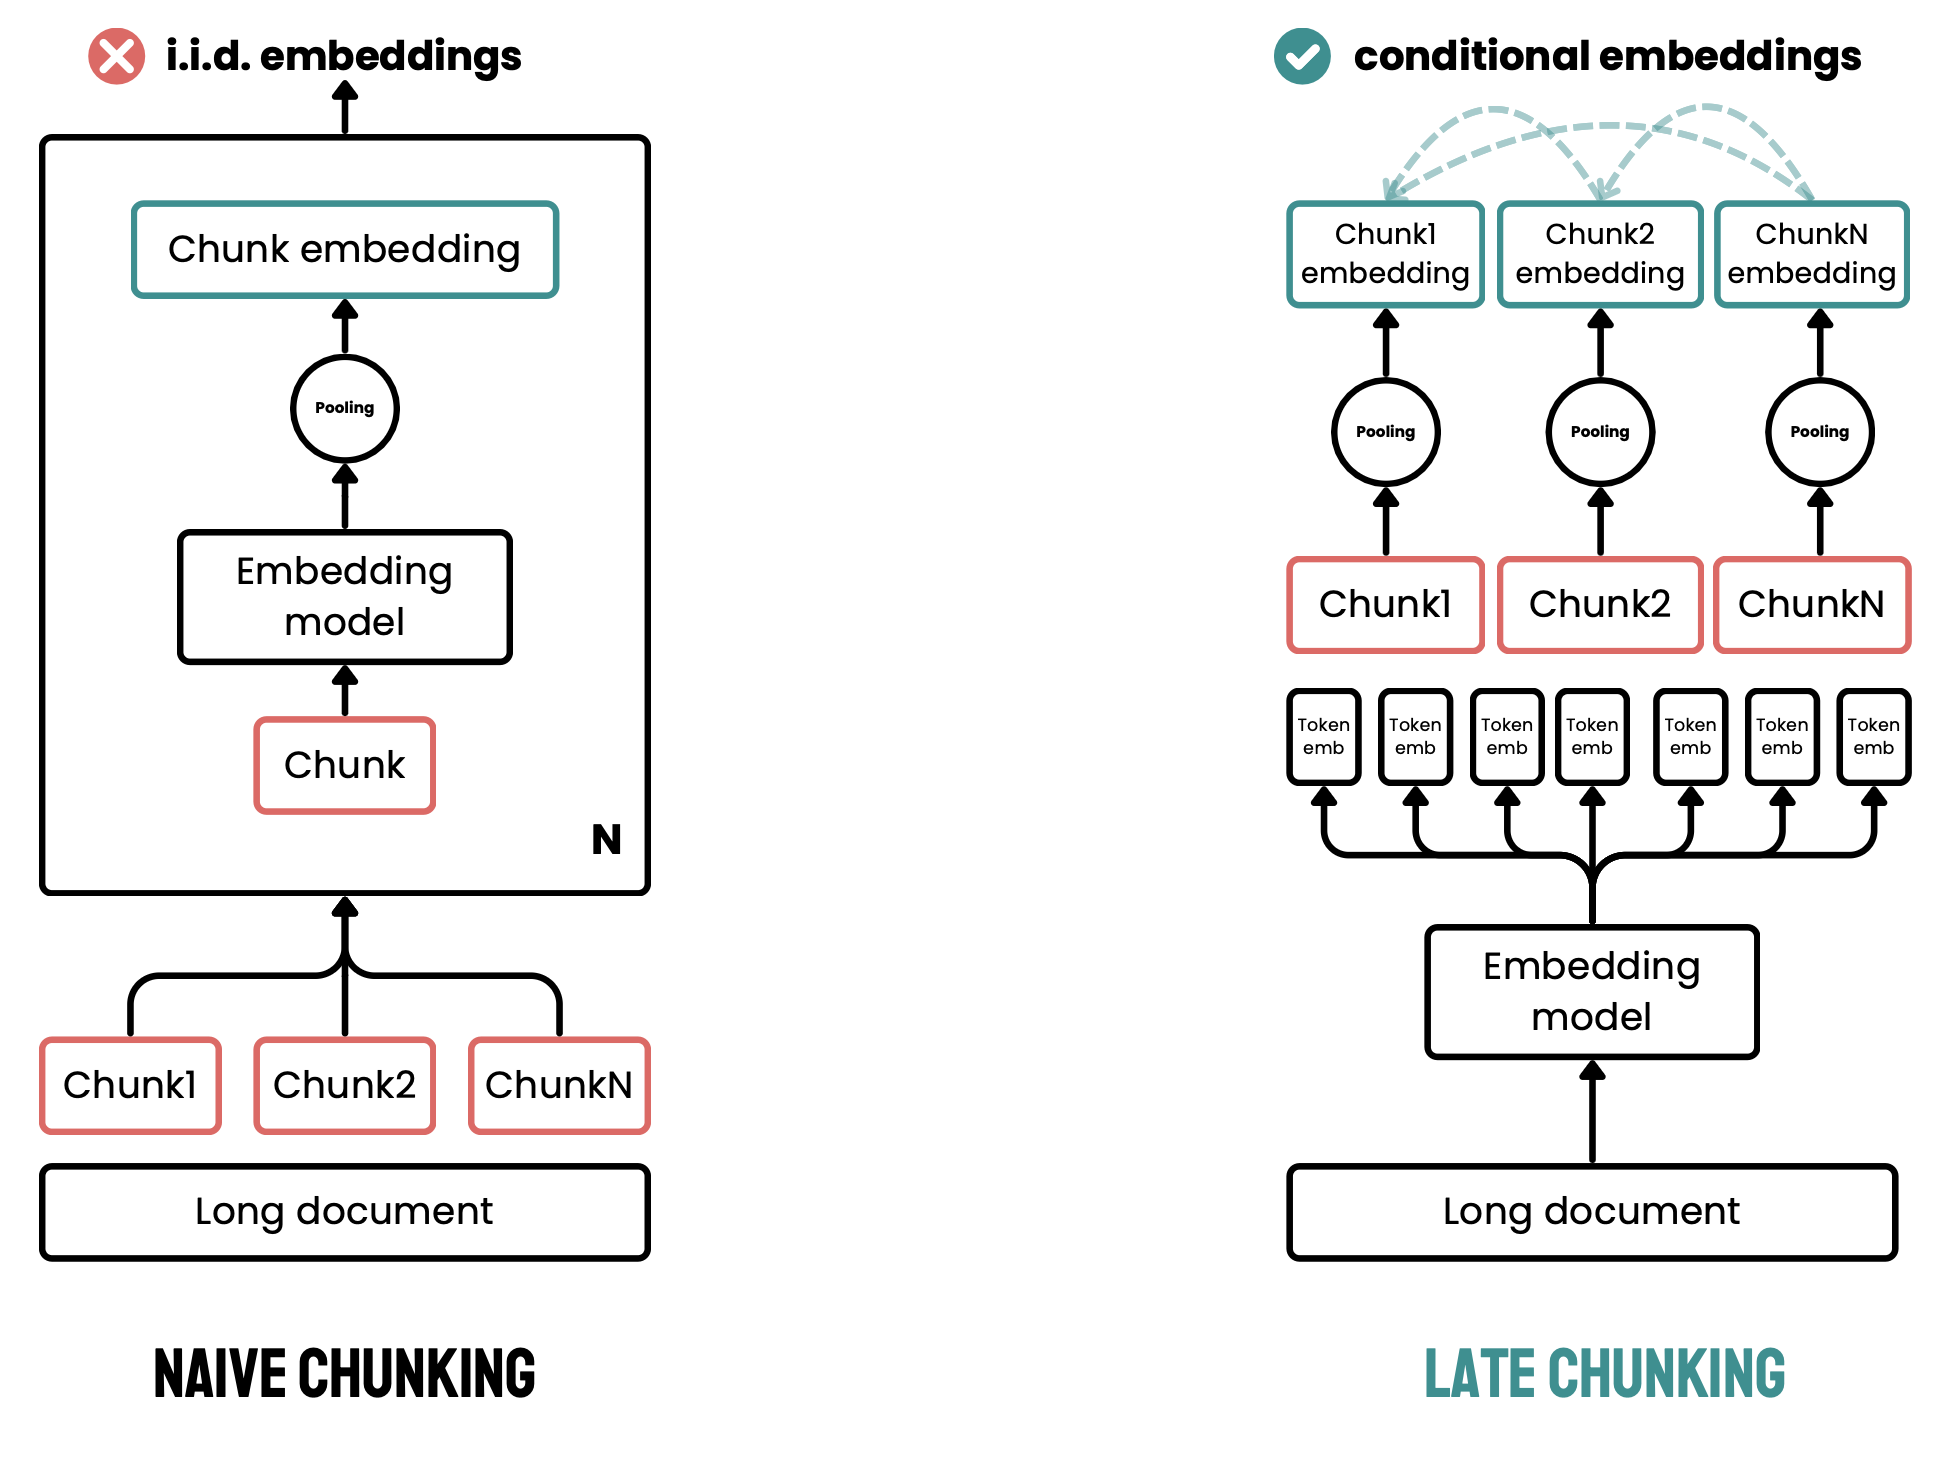
\includegraphics[width=\textwidth]{images/chapter3/late_chunking.png}
    \caption{Visualization of the Late Chunking algorithm (right) compared to naive chunking (left). Image from Günther et al. (2025) \autocite{günther2025latechunkingcontextualchunk}.}
    \label{fig:late_chunking}
\end{figure}

\begin{algorithm}
\caption{Late Chunking}
\label{alg:late_chunking}
\begin{algorithmic}[1]
\Procedure{LateChunking}{document, chunk\_boundaries}
    \State $tokens \gets \text{tokenize}(document)$
    \State $\omega_1, \dots, \omega_m \gets \text{Transformer}(tokens)$ \Comment{Generate token-level embeddings}
    \State $token\_spans \gets \text{get\_token\_spans}(document, tokens)$
    \State $chunk\_token\_indices \gets []$
    \For{each $chunk$ in $chunk\_boundaries$}
        \State $start\_char, end\_char \gets chunk$
        \State $start\_token \gets \text{find\_token\_at\_char}(token\_spans, start\_char)$
        \State $end\_token \gets \text{find\_token\_at\_char}(token\_spans, end\_char)$
        \State append $(start\_token, end\_token)$ to $chunk\_token\_indices$
    \EndFor
    \State $chunk\_embeddings \gets []$
    \For{each $start\_idx, end\_idx$ in $chunk\_token\_indices$}
        \State $token\_vectors\_for\_chunk \gets \omega_{start\_idx}, \dots, \omega_{end\_idx}$
        \State $embedding \gets \text{MeanPool}(token\_vectors\_for\_chunk)$
        \State append $embedding$ to $chunk\_embeddings$
    \EndFor
    \State \Return $chunk\_embeddings$
\EndProcedure
\end{algorithmic}
\end{algorithm}